\documentclass[12pt]{article}
\usepackage{amsmath}
\usepackage{graphicx}
\usepackage{geometry}
\usepackage{indentfirst}
\usepackage{amsfonts}
\geometry{legalpaper, portrait, margin=0.5in}
\usepackage{color}   %May be necessary if you want to color links
\usepackage{hyperref}
\hypersetup{
    colorlinks=true, %set true if you want colored links
    linktoc=all,     %set to all if you want both sections and subsections linked
    linkcolor=black,  %choose some color if you want links to stand out
}
\graphicspath{ {./images/} }
\begin{document}
\newcommand*\dif{\mathop{}\!\mathrm{d}}

\newenvironment{myitemize}
{ \begin{itemize}
    \setlength{\itemsep}{0pt}
    \setlength{\parskip}{0pt}
    \setlength{\parsep}{0pt}     }
{ \end{itemize}                  } 

\newenvironment{myenumerate}
{ \begin{enumerate}
    \setlength{\itemsep}{0pt}
    \setlength{\parskip}{0pt}
    \setlength{\parsep}{0pt}     }
{ \end{enumerate}                  } 

\begin{titlepage}
\begin{center}
\vspace*{2cm}
\begin{huge}\textbf{Machine Learning}\end{huge}
\end{center}
\end{titlepage}

\tableofcontents

\addcontentsline{toc}{section}{Table of contents}

\pagebreak

\section{Regression}

\subsection{Linear regression}
\subsubsection{Squared error cost function}

Measures how well line fits training data

$m$ = num of training examples

$\vec{x}$ holds training example x values (length $m$)

$\vec{y}$ holds training example y values (length $m$)

$\hat y_i$ = $w\vec{x}_i + b$

\[ J(w,b) = \frac{1}{2m} \sum_{i=1}^m ({\hat y}_i - \vec{y}_i)^2 \]

$\frac{1}{m}$ finds average error for larger data sets, $\frac{1}{2m}$ makes later calculations neater

\subsubsection{Gradient descent}

Find $w,b$ for minimum of cost function $J(w,b)$

\begin{myenumerate}
	\item Start with some $w,b$ (commonly $0,0$)
	\item Look around starting point and find direction that will move the point furthest downwards for a small step size
\end{myenumerate}

$\alpha$ = learning rate

Must simultaneously update $w$ and $b$

\begin{align*}
    w_1 &= w_0 - \alpha \frac{\partial}{\partial w} J(w_0,b_0)\\
    b_1 &= b_0 - \alpha \frac{\partial}{\partial b} J(w_0,b_0)\\
    \frac{\partial}{\partial w} J(w,b) &= \frac{1}{m} \sum_{i=1}^m ({\hat y}_i - \vec{y}_i) \vec{x}_i\\
    \frac{\partial}{\partial b} J(w,b) &= \frac{1}{m} \sum_{i=1}^m ({\hat y}_i - \vec{y}_i)
\end{align*}

\subsection{Multiple linear regression}

$n_f$ = number of features

$m$ = number of data points

$\vec{w}$ = vector of weights (length $n_f$)

$X$ is a list of x vectors which hold $n_f$ features (size $m \times n_f$)

Sum of predictions of all features is the prediction of multiple linear reg

\begin{align*}
    f_{\vec{w},b}(\vec{x}) &= \vec{w} \cdot \vec{x} + b
\end{align*}

Gradient descent

\begin{align*}
    \vec{w}_j &= \vec{w}_j - \alpha \frac{\partial}{\partial \vec{w}_j} J(\vec{w},b)\\
    b &= b - \alpha \frac{\partial}{\partial b} J(\vec{w},b)
\end{align*}

Cost function and its partial derivatives

\begin{align*}
    J(\vec{w},b) &= \frac{1}{2m} \sum_{i=1}^{m} (f_{\vec{w},b}(X_i) - \vec{y}_i)^2\\
    \frac{\partial}{\partial \vec{w}_j} J(\vec{w},b) &= \frac{1}{m} \sum_{i=1}^{m} (f_{\vec{w},b}(X_i) - \vec{y}_i) X_{ij}\\
    \frac{\partial}{\partial b} J(\vec{w},b) &= \frac{1}{m} \sum_{i=1}^{m} (f_{\vec{w},b}(X_i) - \vec{y}_i)
\end{align*}

\subsection{Logistic regression}

Sigmoid function

\begin{align*}
    g(z) &= \frac{1}{1 + e^{-z}}\\
    z &= f_{\vec{w},b}(\vec{x})\\
    \hat{y}_i &= g(f_{\vec{w},b}(X_i))
\end{align*}

$\hat{y}_i$ can be interpreted as the "probability" that class is 1, $0 \leq \hat{y}_i \leq 1$

ex. $\hat{y}_i = 0.7$ means there is a 70\% chance $y$ is 1

Logistic regression requires a new cost function because $f_{\vec{w},b}(\vec{x})$ for logistic regression is non-convex, trapping gradient descend in local minima.

Cost function

\[ J(\vec{w},b) = \frac{1}{m} \sum_{i=1}^{m} L(\hat{y}_i,\vec{y}_i) \]

\begin{equation*}
L(\hat{y}_i,\vec{y}_i) = 
  \left\{
    \begin{aligned}
      & -\log(\hat{y}_i) & \text{if } \vec{y}_i = 1 \\
      & -\log(1 - \hat{y}_i) & \text{if } \vec{y}_i = 0
    \end{aligned}
  \right.
\end{equation*}

Simplified form
\[ L(\hat{y}_i, \vec{y}_i) = -\vec{y}_i \log(\hat{y}_i) - (1 - \vec{y}_i) \log (1 - \hat{y}_i) \]

The loss function will decrease as $\hat{y}_i$ approaches $\vec{y}_i$ on a graph of $L$ vs $f$.

$\frac{\partial J(\vec{w},b)}{\partial \vec{w}_j}$ and $\frac{\partial J(\vec{w},b)}{\partial b}$ are the same as in linear regression, just the definition of $f$ has changed.

\subsection{Softmax regression}

Generalization of logistic regression, $y$ can have more than two possible values.

The most probable value of $y$ is the value that when given to $L$ yields the largest loss.

Calculate $z_i$ with $\vec{x}$ only consisting of data points that have label $i$. In implementation, set all $y$ values of data points with label equal to $i$ to 1, and 0 for everything else.

$n_f$ = num features

$n_y$ = number of possible $y$ outputs

$W$ is a matrix of dimensions $n_y \times n_f$.

$\vec{b}$, $\vec{z}$, $\vec{a}$ are vectors of length $n_y$.

\begin{gather*}
    1 \leq i \leq n_y\\
    \vec{z}_i = W_i \cdot \vec{x} + \vec{b}_i\\
    \vec{a}_i = \frac{e^{\vec{z}_i}}{\sum_{k=1}^{n_y} e^{\vec{z}_k}}
\end{gather*}

\begin{equation}
L(\vec{a}, y) =
  \left\{
    \begin{aligned}
    -\log \vec{a}_1 &\text{ if } y = 1\\
    -\log \vec{a}_2 &\text{ if } y = 2\\
    & \vdots\\
    -\log \vec{a}_n &\text{ if } y = n
    \end{aligned}
   \right.
\end{equation}

\subsection{Feature scaling: z-score normalization}

After z-score normalization, all features will have a mean of 0 and a standard deviation of 1

$n_f$ = num features

$\vec{\mu}_j$ = mean of all values for feature $j$ (length $n_f$)

$\vec{\sigma}_j$ = standard deviation of feature $j$ (length $n_f$)

\begin{align*}
    X_{ij} &= \frac{X_{ij} - \vec{\mu}_j}{\vec{\sigma}_j}\\
    \vec{\mu}_j &= \frac{1}{m} \sum_{i=0}^{m-1} X_{ij}\\
    \vec{\sigma}_j^2 &= \frac{1}{m} \sum_{i=0}^{m-1} (X_{ij} - \vec{\mu}_j)^2
\end{align*}

\subsection{Over / underfitting}

Underfit / high bias: does not fit training set well ($wx + b$ fit onto data points with $x + x^2$ shape)

Overfit / high variance: fits training set extremely well but does not generalize well ($w_1 x + w_2 x^2 + w_3 x^3 + w_4 x^4 + b$ fit onto training set of shape $x + x^2$ can have zero cost but predicts values outside the training set inaccurately)

\vspace{5px}

Addressing overfitting
\begin{myitemize}
	\item Collect more data
	\item Select features ("Feature selection")
	\item Reduce size of parameters ("Regularization")
\end{myitemize}

\subsubsection{Regularization}

Small values of $w_1,w_2,\cdots,w_n,b$ for simpler model, less likely to overfit

Given $n_f$ features, there is no way to tell which features are important and which features should be penalized, so all features are penalized.
\[ J_r(\vec{w},b) = J(\vec{w},b) + \frac{\lambda}{2m} \sum_{j=1}^{n_f} \vec{w}_j^2 \]

Can include $b$ by adding $\frac{\lambda}{2m} b^2$ to $J_r$ but typically doesn't make a large difference.

The extra term in $J_r$ is called the regularization term.

Effectively, $\lambda \propto \frac{1}{w}$. When trying to minimize cost, either the error term or the regularization term must decrease. The larger the lambda, the more the regularization term should decrease to minimize cost, decreasing $w$ parameters.

\noindent \textbf{Regularized linear regression}

\[ J_r(\vec{w},b) = \frac{1}{2m} \sum_{i=1}^m \left[(f_{\vec{w},b}(X_i) - \vec{y}_i)^2\right] + \frac{\lambda}{2m} \sum_{j=1}^{n_f} \vec{w}_j^2 \]

For gradient descent, only $\frac{\partial J_r}{\partial \vec{w}_j}$ changes ($b$ is not regularized):

\[ \frac{\partial J_r}{\partial \vec{w}_j} = \frac{1}{m} \sum_{i=1}^m \left[(f_{\vec{w},b}(X_i) - \vec{y}_i)X_{ij}\right] + \frac{\lambda}{m} \vec{w}_j \]

\noindent \textbf{Regularized logistic regression}

\[ J_r(\vec{w},b) = \frac{1}{m} \sum_{i=1}^m L(f_{\vec{w},b}(X_i), \vec{y}_i) + \frac{\lambda}{2m} \sum_{j=1}^{n_f} \vec{w}_j^2 \]

For gradient descent, only $\frac{\partial J_r}{\partial w_j}$ changes (b is not regularized):

\[ \frac{\partial J_r}{\partial \vec{w}_j} = \frac{1}{m} \sum_{i=1}^m \left[(f_{\vec{w},b}(X_i) - \vec{y}_i)X_{ij}\right] + \frac{\lambda}{m} \vec{w}_j \]

\pagebreak

\section{Neural networks}

$n_{\ell}$ = num layers excluding input

$n^{[\ell]}_n$ = n neurons in layer $\ell$

$n_f$ = num features

$\vec{W}$ is a vector (length $n_{\ell}$) of matrices of size $n^{[\ell]}_n \times n^{[\ell-1]}_n$

$\vec{x}$ is a vector of outputs from each neuron in previous layer

$\vec{b}$ is a vector (length $n_{\ell}$), holds a bias value for each layer

$Z$ and $A$: vector (length $n_{\ell}$) of vectors (length $n^{[\ell]}_n$)

$g$: activation function

$1 \leq i \leq n_{\ell}$

$a$ (activation) = scalar output of a single neuron

Superscript $[i]$ is used to notate information relating to the $i$th layer in a neural network.

\subsection{Choosing an activation function}

sigmoid: $g(z) = \frac{1}{1 + e^{-z}}$

tanh: $g(z) = \frac{e^z - e^{-z}}{e^z + e^{-z}}$

linear: $g(z) = z$

ReLU: $g(z) = \max(0, z)$

Leaky ReLU: $g(z) = \max(\epsilon z, z)$ where $\epsilon$ is a small nonzero positive value $<$ 1

\subsubsection*{For output layer}

Binary classification, y = 0 or 1: use sigmoid

Regression, $-\infty \leq y \leq \infty$: use linear activation function

Regression, y $\geq$ 0: use ReLU

\subsubsection*{For hidden layer}

ReLU is most common

\subsection{Training a model}
\subsubsection{Forward propagation}

Input $A^{[\ell-1]}$, output $A^{[\ell]}$, cache $Z^{[\ell]}$, $W^{[\ell]}$, $\vec{b}^{[\ell]}$

\begin{align*}
    Z^{[\ell]} &= W^{[\ell]} A^{[\ell-1]} + \vec{b}^{[\ell]}\\
    A^{[\ell]} &= g^{[\ell]}(Z^{[\ell]})
\end{align*}

Up to $A^{[n_{\ell}]}$, in which case $\hat{y} = A^{[n_{\ell}]}_0$ assuming output layer has one unit

\subsubsection{Back propagation}

Input $\dif a^{[\ell]}$, output $\dif a^{[\ell-1]}$, $\dif W^{[\ell-1]}$, $\dif \vec{b}^{[\ell-1]}$

\begin{align*}
    \dif Z^{[\ell]} &= \dif A^{[\ell]} \cdot g'^{[\ell]}(Z^{[\ell]})\\
    \dif W^{[\ell]} &= \frac{1}{m} \dif Z^{[\ell]} \cdot A^{[\ell-1] T}\\
    \dif \vec{b}^{[\ell]} &= \frac{1}{m} \sum_i \dif Z^{[\ell]}_i\\
    \dif A^{[\ell-1]} &= W^{[\ell] T} \cdot \dif Z^{[\ell]}
\end{align*}

\subsection{Improving model}

Cross validation: split data into training and test, use test data to determine how well the model generalizes

\subsubsection{Fixing high bias/variance}

High bias (underfit): $J_{train}$ high, $J_{train} \approx J_{cv}$

High variance (overfit): $J_{train}$ may be low, $J_{cv} \gg J_{train}$

High bias and high variance: $J_{train}$ high, $J_{cv} \gg J_{train}$

How to fix:

\begin{myenumerate}
\item Get more training examples (fix high variance)
\item Try smaller sets of features (fix high variance)
\item Add more features (fix high bias)
\item Add polynomial features (fix high bias)
\item Decrease $\lambda$ (fix high bias)
\item Increase $\lambda$ (fix high variance)
\end{myenumerate}

\textbf{Neural networks and bias/variance}

If $J_{train}$ is high, make the network larger

If $J_{cv}$ is high, get more data

\subsubsection{Adding data}

Data augmentation: add data with distortions (ex. distorted letters in a letter recognition program)

\section{Decision trees}

\subsection{Measuring purity}

\subsubsection{Entropy as a measure of impurity}

$p$ = fraction of examples that are cats

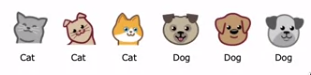
\includegraphics{purity}

$p$ = $\frac{1}{2}$

Impurity can be measured with the entropy function $H(p)$

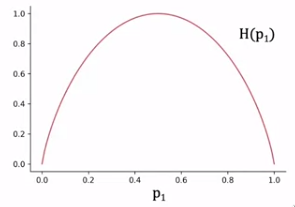
\includegraphics{entropy}

Higher $H$ = less pure, more information gain

Mathematically, $H$ is defined as:

\begin{align*}
    H(p) &= -p \log_2(p) - (1 - p) \log_2(1 - p)
\end{align*}

$0 \log(0)$ is defined as 0 for the function $H$

\subsection{Choosing a split}

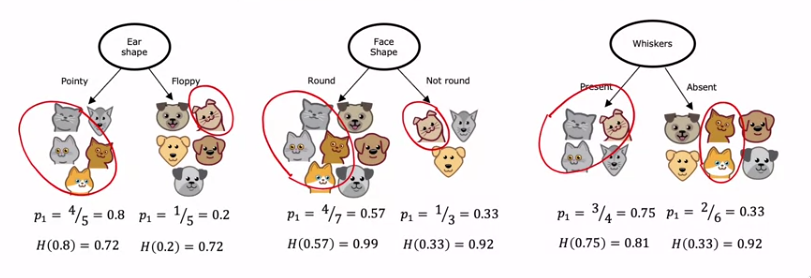
\includegraphics[scale=.6]{split}

To choose which feature to split data on is the best, calculate the weighted average of the entropy on the left
and right branches, then choose which split has the highest entropy (least pure, which will give a good split).\\

Average of ear shape split entropy: $0.5 H(0.8) + 0.5 H(0.2) = 0.28$

Average of face shape split entropy: $0.7 H(0.57) + 0.3 H(0.33) = 0.03$

Average of whiskers split entropy: $0.4 H(0.75) + 0.6 H(0.33) = 0.12$

Ear shape has the largest entropy, so the best choice is to split based on ear shape.\\

Formal definition of information gain:

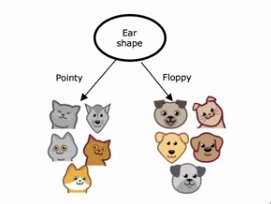
\includegraphics{information-gain}

$p_{root}$ = percentage of positive examples (0.5 in this case)

$p_{left}$ = 4/5

$p_{right}$ = 1/5

$w_{left}$ = 5/10

$w_{right}$ = 5/10

$H(p_{root}) - (w_{left} H(p_{left}) + w_{right} H(p_{right}))$

\subsection{Constructing a decision tree}

\begin{myenumerate}
    \item Start with all examples at root node
    \item Calculate information gain for all possible features, pick one with highest information gain
    \item Split dataset according to selected feature, creating a left and right branch
    \item Stop when stopping criteria is met (node is 100\% one class, information gain
        from more splits is less than a threshold, num examples is below a threshold)
\end{myenumerate}

Final decision tree

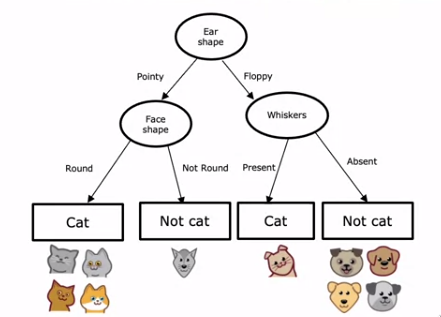
\includegraphics[scale=.5]{decision-tree}

\subsection{Features with multiple possible values}

\textbf{Known number of possible values}

If a categorical feature can take on $k$ values, create $k$ binary features

ex. Create a true/false feature for pointy ears, floppy ears, and oval ears instead of a single
feature "ear shape" which takes on three possible values.\\

\textbf{Unknown number of possible values}

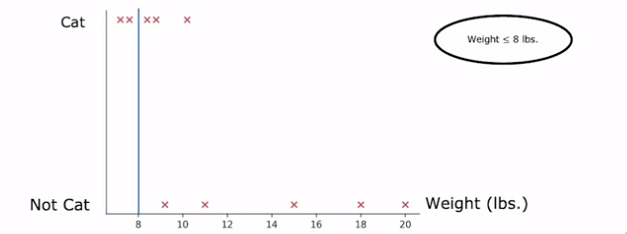
\includegraphics[scale=.7]{continuous-tree}

Split on weight $\le$ 8 lbs

$p_{root}$ = 0.5

$p_{left}$ = 1

$p_{right}$ = 3/8

$w_{left}$ = 2/10

$w_{right}$ = 8/10

$H(0.5) - (\frac{2}{10} H(1) + \frac{8}{10} H(\frac{3}{8}))$

To find most optimal information gain (maximize $H$), make splits between every pair of adjacent data points and choose
the one with the highest information gain.

\subsection{Tree ensembles}

Training multiple decision trees will lead to more accurate predictions since
a single decision tree is sensitive to small changes in data.

\subsubsection{Sampling with replacement}

Take original training set of size $m$ and randomly select from the original training set to
create a new training set of size $m$. Repeated data is expected.

This will create new datasets that are similar to the original dataset, but are slightly different
which will create unique decision trees.

\subsubsection{Random forest algorithm}

From $b$ = 1 to $B$: sampling with replacement to create new dataset, train decision tree on new dataset.

$B$ is commonly around 100. Setting $B$ too large doesn't hurt performance but gives diminishing returns
as it increases.\\

Randomizing feature choice is another way to create more unique decision trees:
Given $n$ features, give each decision tree a subset of all features of size $k$.

A good value for $k$ is $k = \sqrt n$.

\subsubsection{XGBoost}

Instead of picking from all training data with equal probability in the random forest algorithm,
make it more likely to pick misclassified examples from previous decision trees

\section{Unsupervised learning}

\subsection{Clustering: K-means}

\subsubsection{Algorithm}

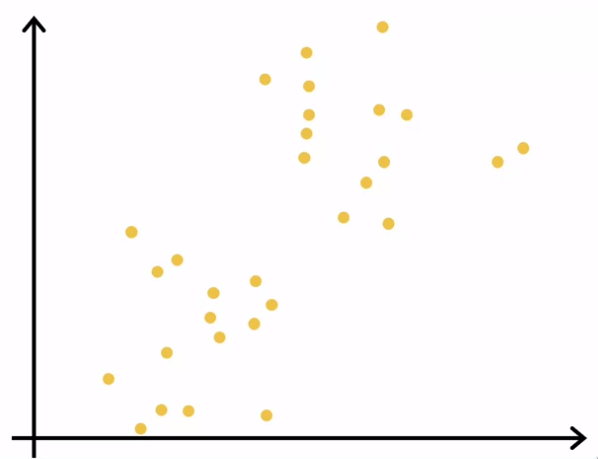
\includegraphics[scale=.5]{images/clusters.png}

Given a dataset like this, the algorithm will guess the centers of
two different clusters (Determining number of clusters will be covered later).

Once two cluster centers (or centroids) are guessed, each data point on the graph
will be associated with the centroid it's closest to. The centroid will then move to
the average position of all its data points.

Eventually, the centroids will move to the center of the two clusters:

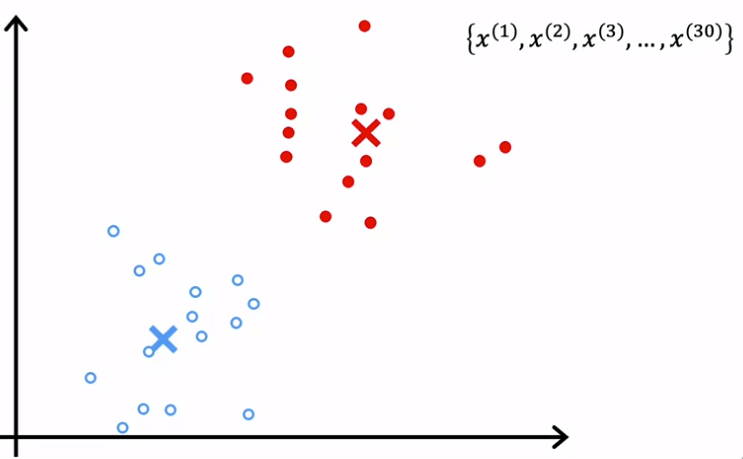
\includegraphics[scale=.5]{images/cluster-finished.png}

\subsubsection{Cost function}

$k$ = num clusters

$\vec{c}_i$ = index of cluster (1,2,$\ldots$,$k$) to which example $\vec{x}_i$ is currently assigned

$\mu_i$ = cluster centroid $i$

$\mu_{\vec{c}_i}$ = cluster centroid of cluster to which example $\vec{x}_i$ is currently assigned to

\[ J(\vec{c},\vec{\mu}) = \frac{1}{m} \sum_{i=1}^m \| \vec{x}_i - \vec{\mu}_{\vec{c}_i} \|^2 \]

The cost function can be used to determine how well the centroids predicted the clusters, and it can
also determine when k-means is converging.

The most optimal centroids can be determined by running k-means multiple times with random initial centroid
positions every time, then choosing the result with the lowest cost.

\subsubsection{Choosing k}

\textbf{Elbow method}

Plot cost as a function of $k$, choose $k$ where cost begins to decrease at a slow rate.

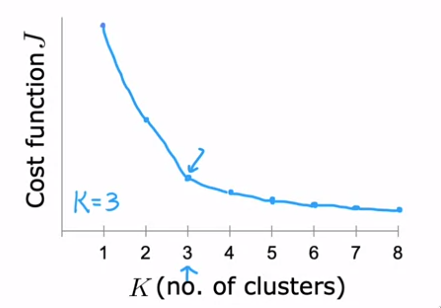
\includegraphics[scale=.6]{elbow}

In this graph, $k$ = 3 might be a good number of clusters. Although cost does continue to decrease as $k$ increases
beyond 3, the number of clusters is too large and makes for less meaningful clusters.

The "right" value of $k$ is often ambiguous however, which is an issue with the elbow method.

\subsection{Anomaly detection}

\subsubsection{Normal distribution}

The equation for the normal distribution is given by

\[ p(x,\mu,\sigma) = \frac{1}{\sqrt{2\pi}\sigma} e^{\frac{-(x - \mu)^2}{2\sigma^2}} \]

Change in $\mu$ will shift the curve on the x axis, and change in $\sigma$ will make the curve
thinner or wider. Smaller $\sigma$ makes curve narrow, larger $\sigma$ makes curve wide.

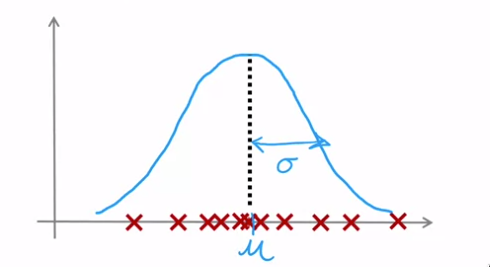
\includegraphics{images/normal-distribution.png}

Values of $\mu$ and $\sigma$ that produce a normal distribution which will fit the data well can be determined
like this:

\begin{align*}
    \mu &= \frac{1}{m} \sum_{i=1}^m \vec{x}_i\\
    \sigma^2 &= \frac{1}{m} \sum_{i=1}^m (\vec{x}_i - \mu)^2
\end{align*}

\subsubsection{Density estimation}

Training set: matrix $X$ of size $m \times n$ ($m$ examples, $n$ features)

\[ p(\vec{x}) = \prod_{i=1}^n p(\vec{x}_i,\mu_i,\sigma_i^2) \]

\subsection{Recommender systems}

$n$ = num features

$n_i$ = num items

$r(i,j) = 1$ if user $j$ has rated item $i$ (0 if otherwise)

$y_{i,j}$ = rating given by user $j$ on item $i$ (if defined)

$W_j,\vec{b}_j$ = parameters for user $j$

$X_i$ = feature vector for item $i$

$\vec{m}_j$ = number of items user $j$ has rated

For user $j$, predict rating of item $i$ with $W_j \cdot X_i + \vec{b}_j$

Feature example:

\begin{center}
    \begin{tabular}{ ||c|c|c|c|| }
        \hline
        Movie & $X_{i1}$ (Romance) & $X_{i2}$ (Action) & $X_{i3}$ (Horror)\\
        \hline
        Romance movie ($i$ = 1) & 1.0 & 0.1 & 0.0\\
        Action movie ($i$ = 2) & 0.0 & 1.0 & 0.0\\
        Comedy movie ($i$ = 3) & 0.5 & 0.0 & 0.0\\
        Horror movie ($i$ = 4) & 0.0 & 1.0 & 1.0\\
        \hline
    \end{tabular}
\end{center}

Cost function to learn parameters for user $j$:

\[ J(W_j,\vec{b}_j) = \frac{1}{2\vec m_j} \sum_{i:r(i,j)=1} (\vec w_j \cdot X_i + \vec b_j - y_{i,j})^2 \]

Learn parameters for all users $n_u$:

$W$ is a matrix of size $n_u \times n$

$\vec{b}$ is a vector of length $n_u$

\[ J(W,\vec{b}) = \frac{1}{2} \sum_{j=1}^{n_u} \left[ \sum_{i:r(i,j)=1} (\vec{w}_j \cdot X_i + \vec b_j - y_{i,j})^2 \right] \]

\subsubsection{Collaborative filtering}

Given user parameters $\vec{w}$ and $b$, predict features.

To learn $X_i$:

\[ J(X_i) = \frac 1 2 \sum_{j:r(i,j)=1} (\vec w_j \cdot X_i + \vec b_j - y_{i,j})^2 \]

To learn $X_{1 \ldots n_m}$:

\[ J(X) = \frac 1 2 \sum_{i=1}^{n_m} \sum_{j:r(i,j)=1} (\vec w_j \cdot X_i + \vec b_j - y_{i,j})^2 \]

\subsubsection{Cost function}

\[ J(\vec w, \vec b, X) = \frac 1 2 \sum_{(i,j):r(i,j)=1} (\vec w_j \cdot X_i + \vec b_j - y_{i,j})^2 \]

\subsubsection{Binary labels}

Predict probability of $y_{i,j}$ = 1 using $a_{i,j} = g(\vec w_j \cdot X_i + \vec b_j)$ where $g(z) = \frac 1 {1 + e^{-z}}$

Loss for binary labels

\[ L(a_{i,j},y_{i,j}) = -y_{i,j} \log(a_{i,j}) - (1 - y_{i,j}) \log(1 - a_{i,j}) \]

Cost function

\[ J(\vec w, \vec b, X) = \sum_{(i,j):r(i,j)=1} L(g(\vec w_j \cdot X_i + \vec b_j),y_{i,j}) \]

\subsubsection{Mean normalization}

Allows the algorithm to give better predictions for users who have rated very few movies.

Given a chart like this,

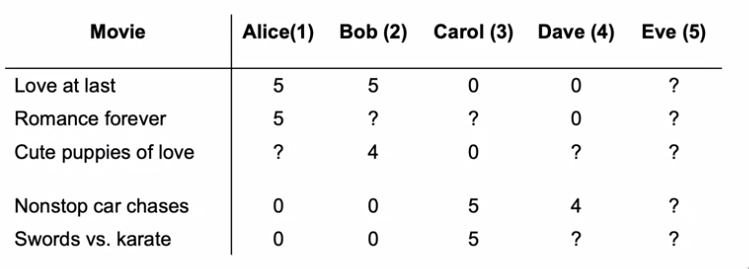
\includegraphics[scale=.5]{movies}

create a matrix

\[
\begin{bmatrix}
    5 & 5 & 0 & 0 & ?\\
    5 & ? & ? & 0 & ?\\
    ? & 4 & 0 & ? & ?\\
    0 & 0 & 5 & 4 & ?\\
    0 & 0 & 5 & ? & ?
\end{bmatrix}
\]

\[
    \mu =
    \begin{bmatrix}
        2.5\\
        2.5\\
        2\\
        2.25\\
        1.25
    \end{bmatrix}
\]

After subtracting every value in each row by its corresponding $\mu$:

\[
    \begin{bmatrix}
        2.5 & 2.5 & -2.5 & -2.5 & ?\\
        2.5 & ? & ? & -2.5 & ?\\
        ? & 2 & -2 & ? & ?\\
        -2.25 & -2.25 & 2.75 & 1.75 & ?\\
        -1.25 & -1.25 & 3.75 & -1.25 & ?
    \end{bmatrix}
\]

\subsubsection{Finding related items}

Find item $k$ with $X_k$ similar to $X_i$

\[ \sum_{l=1}^n (X_{k,l} - X_{i,l})^2 \]

\subsubsection{Content based filtering}

Recommends items user might like, in contrast to collaborative filtering which decides if a user
would like an item

\end{document}
